\section{提案手法}


\begin{figure}[htbp]
  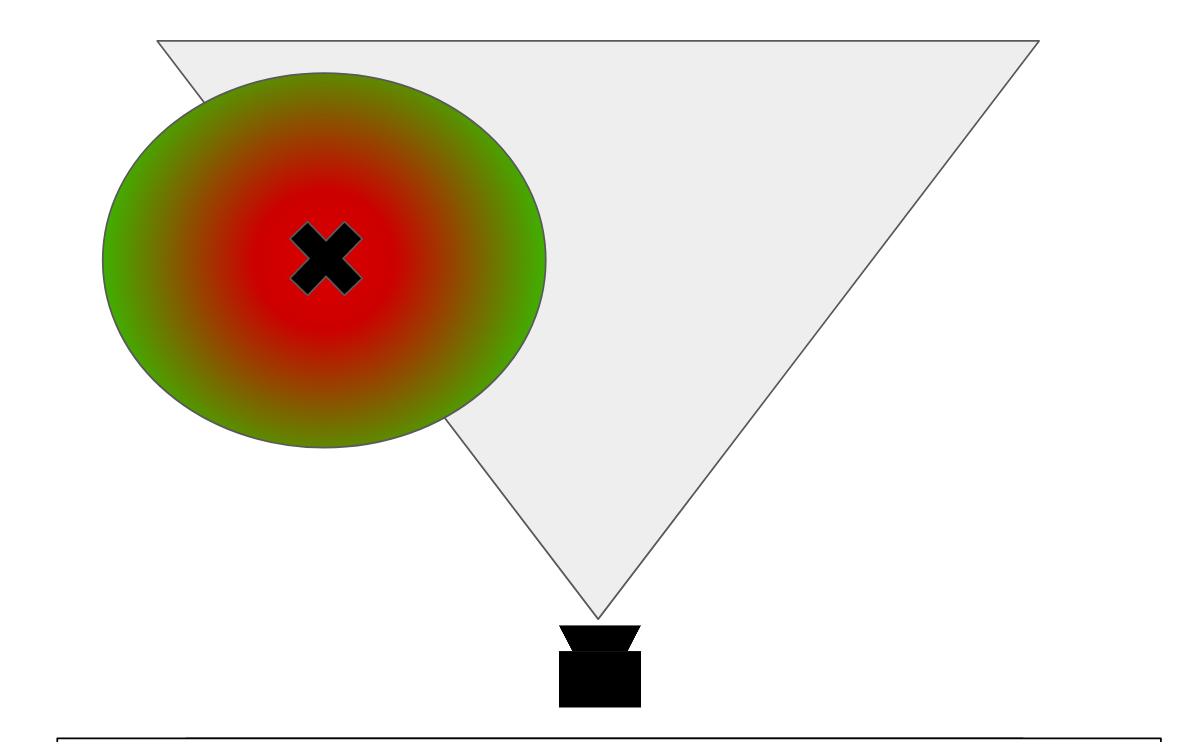
\includegraphics[width=7cm]{img/figure1.png}
  \caption{動く可能性の低い物体}
\end{figure}
\begin{figure}[htbp]
  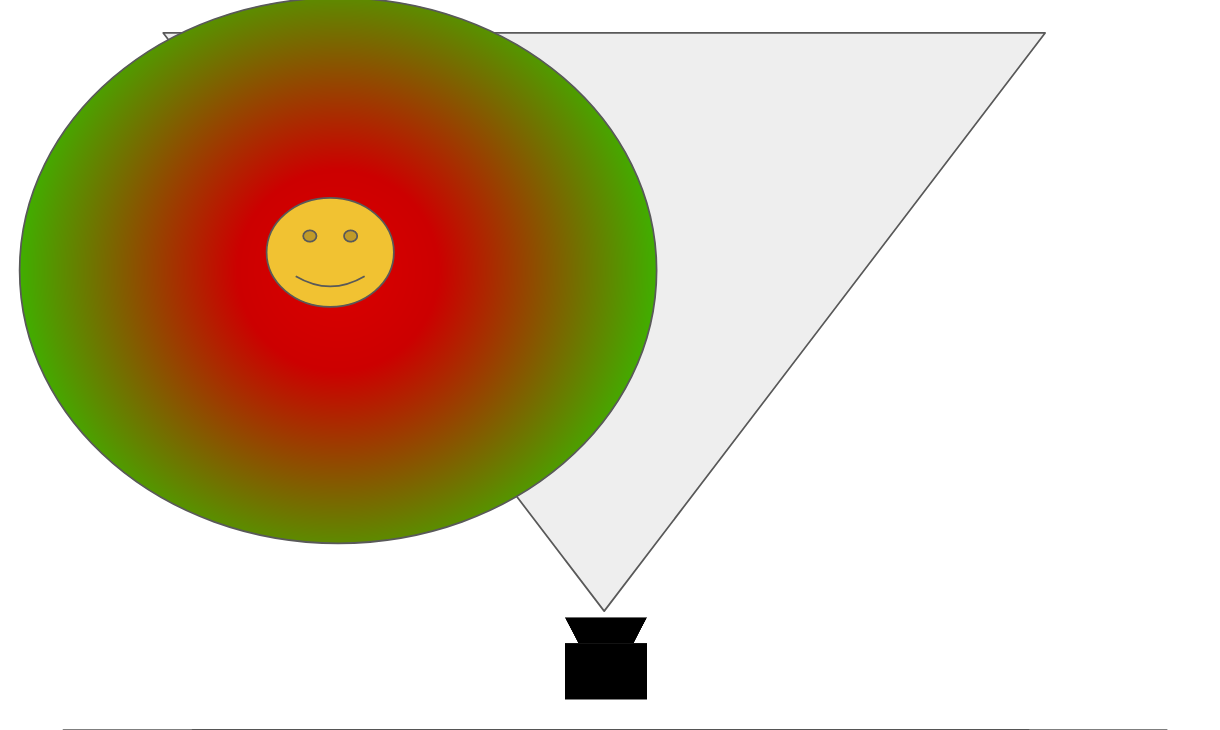
\includegraphics[width=7cm]{img/figure2.png}
  \caption{動く可能性の高い物体}
\end{figure}

まず,1つ目の飛行経路探索を行う処理系に関しては以下の条件を判断軸にして経路選択,飛行を行うものとする

\begin{enumerate}
\item 視野の中に映る検出された物体の中で画面占有率の高いものをより重要度が高いものとして設定する.
\item 検出される物体が一番少ない何もない所を一番安全な方向として設定する.
\item 何も検出されなくなった場合,大きな平面に直面したとして一時停止する.
\end{enumerate}

次に2つ目の検出した物体の属性を判定する部分であるが,こちらは検出時にラベルが得られるのでそのラベルをキーとして辞書データから検出する事とする.
また,おおよその移動速度も物によって推測でき,辞書データの中に含める事で,排他的空域をどこまで広げるかを設定する.
動くことが想定される物体よりも高い位置で飛ぶ際もその直上は落下可能性を拭いきれないので飛行禁止空域として設定する.

実際に使用する技術としては以下のものの使用を考えている.
\begin{itemize}
\item Tello
\item MacBookPro 2016Model
\item Yolo v3
\end{itemize}
